%%%%%%%%%%%%%%%%%%%%%%%%%%%%%%%%%%%%%%%%%%%%%%%%%%%%%%%%%%%%%%%%%%%%%%%%%%%%%%%%
%2345678901234567890123456789012345678901234567890123456789012345678901234567890
%        1         2         3         4         5         6         7         8

\documentclass[letterpaper, 10 pt, conference]{ieeeconf}  % Comment this line out if you need a4paper

%\documentclass[a4paper, 10pt, conference]{ieeeconf}      % Use this line for a4 paper

\IEEEoverridecommandlockouts                              % This command is only needed if 
                                                          % you want to use the \thanks command

\overrideIEEEmargins                                      % Needed to meet printer requirements.

\usepackage{lipsum} % for dummy text
\usepackage{scrextend} % for footnote with multiple references
\usepackage[pdftex]{graphicx} % graphics package
\usepackage[caption=false]{subfig} % subplot package
\usepackage{siunitx} % package for international system units
\usepackage{multirow} % multiple rows in table
\usepackage{array} % fixed size of columns in tables
\let\labelindent\relax\usepackage{enumitem} % for cross-reference in the bullet-points list
\usepackage{color} % colors package
\usepackage{colortbl} % for colors in tables
\usepackage{pifont} % for check-mark and X-mark
\usepackage{amsmath} % for bold symbols
\usepackage{amssymb}
\usepackage{dblfloatfix} % to place floats on the bottom of the page
\usepackage[ruled,vlined,resetcount]{algorithm2e}
\usepackage[caption=false,font=footnotesize]{subfig}
\usepackage{tikz}
\usetikzlibrary{shapes, arrows, fit, calc, positioning, automata, decorations.markings, backgrounds}
\tikzset{>=latex}

\setcounter{MaxMatrixCols}{20} % for huge matrices and vectors

\makeatletter
\let\NAT@parse\undefined
\makeatother
\PassOptionsToPackage{hyphens}{url}
\usepackage[colorlinks=true,linkcolor=blue,urlcolor=blue,citecolor=blue,anchorcolor=blue]{hyperref} % hyperlink package (needs to be put at the end!)

\graphicspath{{figures/}} % declare the path where graphic files are

\newtheorem{theorem}{Theorem}
\newtheorem{corollary}{Corollary}
\newtheorem{lemma}{Lemma}
\newtheorem{definition}{Definition}
\newtheorem{remark}{Remark}
\newtheorem{assumption}{Assumption}

\newcommand{\argmin}[1]{\underset{#1}{\operatorname{arg}\,\operatorname{min}}\;}
\newcommand{\argmax}[1]{\underset{#1}{\operatorname{arg}\,\operatorname{max}}\;}

\title{\LARGE \bf
Dynamic System Emulation: Fixed Wing Dynamics on a Multicopter
}

\author{Abdelhakim Amer$^{1}$ and Andriy Sarabakha$^{1}$% <-this % stops a space
\thanks{This research was supported by the Aarhus University Research Foundation.}
\thanks{$^{1}$Abdelhakim Amer and Andriy Sarabakha are with the Department of Electrical and Computer Engineering, Aarhus University, Denmark. {\tt\small \{abdelhakim, andriy\}@ece.au.dk}}%
}

\begin{document}

\bstctlcite{IEEEexample:BSTcontrol}

\maketitle
\thispagestyle{empty}
\pagestyle{empty}
% \thispagestyle{plain}
% \pagestyle{plain}

%%%%%%%%%%%%%%%%%%%%%%%%%%%%%%%%%%%%%%%%%%%%%%%%%%%%%%%%%%%%%%%%%%%%%%%%%%%%%%%%
%%%%%%%%%%%%%%%%%%%%%%%%%%%%%%%%%%%%%%%%%%%%%%%%%%%%%%%%%%%%%%%%%%%%%%%%%%%%%%%%
%%%%%%%%%%%%%%%%%%%%%%%%%%%%%%%%%%%%%%%%%%%%%%%%%%%%%%%%%%%%%%%%%%%%%%%%%%%%%%%%
\begin{abstract}

This work presents a control framework that enables a multicopter equipped with a two-axis gimbal to emulate the flight dynamics of a fixed-wing aircraft. The goal is to provide an operationally simple platform for training and simulation that avoids the aerodynamic constraints of fixed-wing vehicles, such as minimum airspeed and nonholonomic constraints.
A state-input mapping between the two platforms is derived using dynamic feedback linearization. %The mapping yields a fourth-order translational chain and a second-order heading chain, allowing the multirotor to track trajectories produced by a virtual fixed-wing model. To maintain performance near actuator and model limits, we introduce an authority-aware geometric damping augmentation that applies geometric PD-style attitude damping and proportionally scales outer-loop demands to avoid divergence under low-authority conditions.
The framework is evaluated on representative fixed-wing manoeuvres. %Tracking performance is quantified via translational mean absolute error and attitude geodesic error between the fixed-wing reference and the quadcopter–gimbal system. 
Results show high-fidelity emulation under nominal conditions. While evaluations are conducted in simulation, the approach establishes a practical path toward hardware deployment for pilot training, autonomy research, and controller benchmarking.

\end{abstract}

%%%%%%%%%%%%%%%%%%%%%%%%%%%%%%%%%%%%%%%%%%%%%%%%%%%%%%%%%%%%%%%%%%%%%%%%%%%%%%%%
%%%%%%%%%%%%%%%%%%%%%%%%%%%%%%%%%%%%%%%%%%%%%%%%%%%%%%%%%%%%%%%%%%%%%%%%%%%%%%%%
%%%%%%%%%%%%%%%%%%%%%%%%%%%%%%%%%%%%%%%%%%%%%%%%%%%%%%%%%%%%%%%%%%%%%%%%%%%%%%%%


\section{Introduction}

% %%Hakim Comments
% %%A) Motivation
% %% Add motivation: Why emulation is needed? 
% % 1. Fixed wings aircrafts are more expensive, not widely accessable 
% % 2. One system can mimic a wide variety of vehicles ( VTOL's different aircraft models)
% % 3. Can be used for training pilots
% % 4. Viewpoint equivalence: for perception algorithms the image stream will be indistinguishable
% % 5. Algorithm validation at lower TRL
% % Why drone-gimbal system? drone-gimbal system is an accessible adn cheap platform for emulation.
% % 4. Photorealistic simulators

% %%B) Applications
% %% Add examples of emulation for aircraft systems, give examples of flight and driving simulators, examples for industry and academdia, for example SIMONA at TU Delft. (add citations)


% %% C) Advanced Control Methods for dynamcis mimecry  why DFL? (add citations).

% % cite DFL methods, andriys thesis and paper on relative degree, mohits paper
% % cite differet contorl methods, ex. MPC and limitations





% % Motivation
% %Mimicking one dynamic system with another can enable low-cost, safe, and repeatable testing and data collection, algorithm validation, operational flexibility across environments, and output equivalence for perception-driven tasks without the logistical or risk of the target platform.

% The increasing complexity and cost of controlling specific dynamical systems, such as fixed-wing aircraft, pose significant challenges in training, simulation and real-world operations. Fixed-wing platforms are constrained by aerodynamic principles that limit their manoeuvrability. As they cannot hover or fly sideways, they must maintain a minimum airspeed, and their stability margins depend significantly on flight conditions ~\cite{morando2025trajectory}. These constraints make fixed-wing systems demanding in both operation and replication in controlled environments~\cite{li2024high}. By contrast, quadcopters are mechanically simpler, more affordable, and much more maneuverable. They can hover, fly laterally, and execute aggressive manoeuvres within confined spaces, making them attractive candidates for mimicking the behaviour of a more complex aerial system. If a quadcopter emulated the dynamics of a fixed-wing aircraft, it would open up practical applications in low-cost training, simulation and autonomy research. %For example, a quadcopter equipped with a gimbal-mounted camera could reproduce fixed-wing trajectories for pilot training or algorithm validation without requiring access to a real fixed-wing aircraft. 

% % Challenges
% Despite this potential, emulating one aerial system with another presents several significant challenges. The dynamics of fixed-wing aircraft and quadcopter vehicles differ fundamentally; one relies on continuous forward motion to generate lift, while the other produces lift through vertical thrust. Nonholonomic constraints, aerodynamic stall behaviour, differences in actuation and stability characteristics all make direct mapping between the two systems complex. A practical solution must therefore include a rigorous mechanism that can analyse the similarities between the two systems, derive mappings between their states and inputs, and ensure that the secondary system (multicopter) accurately mimics the primary system (fixed-wing aircraft) under realistic flight conditions ~\cite{yuan2025design, wu2019modeling}.

% % Related works
% In~\cite{wang2023similarity}, a framework is presented to measure similarity between two dynamic systems. It defines a homeomorphic map $K$ that transforms the trajectories of one system to match those of another, and quantifies the fidelity of the transformation via a cost function $J[K]$. The minimiser $K^*$ is used to minimise the cost, including the existence, uniqueness, and maximum principles, which provide a rigorous foundation for a similarity measure between two dynamical systems. Additionally, the paper introduces a ’similarity degree’ metric, which allows for classification of similarity in rigid, linear and general forms depending on the nature of $K^*$. It also demonstrates the practical viability of this approach through simulations of chaotic systems, such as Lorenz's and Chua’s circuits. 



% % Contribution
% The objective of this work is to design and validate a framework that enables a quadcopter with a two-axis gimbal to emulate the dynamics of a fixed-wing aircraft. Specifically, the work seeks to model and compare the key dynamical properties of both systems, develop a mapping strategy between their states and inputs, based on dynamic feedback linearization~(DFL) and design control laws that allow the quadcopter to mimic fixed-wing trajectories, and validate the framework through simulation to assess the accuracy and robustness ~\cite{pollet2022common} through increasingly complex maneuvers. The open-source implementation of the proposed framework is available \footnote{Repository: \url{https://github.com/abdelhakim96/Ghost_Tracking_DFL}}





% % Organisation
% This manuscript is organised as follows. The preliminary information about the fixed-wing and multicopter aircraft is summarised in Section~\ref{sec:preliminaries}. Section~\ref{sec:proof} provides a proof of full controllability of the camera's pose mounted on a multicopter's gimbal and a proof of fixed-wing aircraft camera pose mimicry with a multicopter's camera. Section~\ref{sec:method} proposes a method for the dynamic system imitation. Section~\ref{sec:results} provides validation results. Finally, the conclusions are provided in Section~\ref{sec:conclusions}.



% % A) Taxonomy of Emulation
% Mimicking the behaviour of one dynamical system with another, a process broadly
% termed emulation, is a powerful tool in engineering and research. These
% approaches can be classified into a taxonomy based on their connection to the
% real world. The first category is purely virtual Simulation, where a
% computer model replicates a system's dynamics and its sensory environment. The
% second is hardware-in-the-Loop simulation, which combines a physical motion
% platform with a virtual environment. The third, which is the focus of this work,
% is system-to-system emulation, where one real-world physical system is
% controlled to dynamically replicate another.


% % B) Type 1: Purely Virtual (AirSim)
% Purely virtual simulators, which leverage game engines like
% Unreal Engine \cite{shah2017airsim, amer2023unav}, are designed to generate vast amounts of synthetic sensor data to
% train perception algorithms~\cite{shah2017airsim}. While valuable for rapidly
% testing code and training models, these systems suffer from the well-known
% "sim-to-real gap"~\cite{gao2020realitygap}. Models trained purely on simulated
% data often fail when deployed on a real robot because the simulation cannot
% perfectly capture the noise, lighting, and unpredictable dynamics of the real
% world.

% % C) Type 2: Physical-in-the-Loop (SIMONA)
% Hardware-in-the-Loop simulators seek to add realism by incorporating a human
% operator and physical motion cues. Advanced research platforms, like the SIMONA
% simulator at TU Delft, use a stewart platform to
% provide realistic motion feedback for pilot training~\cite{vanpaassen2006simona,
% stroosma2002simona}. However, these systems are ultimately disconnected from the
% real world. The visual feedback is still a computer-generated image, creating a
% validation gap for both the pilot and any onboard sensor-driven algorithms.

% % D) Type 3: Physical-to-Physical (Our Paradigm)
% This work introduces a framework for the third paradigm: physical-to-physical
% system emulation. We propose using one highly-maneuverable, low-cost physical system (a
% quadcopter with a gimbal) to emulate the dynamics and camera viewpoint of
% another, more constrained physical system (a fixed-wing aircraft).

% This approach bridges the gap left by the other methods. For algorithm validation, it provides
% a real-time, real-world video stream, eliminating the "sim-to-real gap" by
% incorporating actual environmental physics. For pilot training, it provides a
% visual feed that is "actually real, not kind of real," offering a transformative
% tool for training in real-world conditions without risking a high-value
% fixed-wing asset.

% % E) Problem Statement & Advantages
% The specific problem we address is emulating a fixed-wing aircraft, a platform
% that is costly and challenging to operate due to its aerodynamic constraints
% (e.g., minimum airspeed, limited maneuverability). A quadcopter is an ideal
% emulation platform due to its affordability and maneuverability (e.g., hovering,
% lateral flight). This capability is crucial for validating algorithms at lower
% Technology Readiness Levels (TRLs)~\cite{smith2022emulation} and enables
% flexible, repeatable data collection for perception tasks.

% % F) Challenges (Transition to Control)
% Achieving this emulation, however, presents a significant control challenge. The
% dynamics of fixed-wing aircraft and quadcopters differ fundamentally. Mapping the
% nonholonomic constraints, aerodynamic stall behaviours, and disparate actuation
% models from the fixed-wing (primary) system to the quadcopter (secondary) system
% is highly non-trivial. A practical solution requires a rigorous control framework
% that can derive precise mappings between their states and inputs, ensuring the
% quadcopter accurately reproduces the fixed-wing's behaviour under realistic flight
% conditions~\cite{yuan2025design, wu2019modeling}.

% % G) Advanced Control Methods (Related Work - Control)
% To achieve this dynamic mimicry, advanced control methods are essential.
% Model predictive control (MPC) is one popular approach, valued for its
% ability to handle system constraints and optimize trajectories~\cite{amer2023visual,amer2025}.
% However, MPC's high computational cost can be a significant limitation for
% real-time applications on embedded hardware. An alternative and highly effective
% strategy is dynamic feedback linearization (DFL). DFL-based control uses, when
% necessary, a dynamic extension of the state space to transform the complex
% nonlinear system dynamics into a simpler, linear form. This allows for systematic
% and computationally efficient trajectory tracking, and it is a powerful tool for
% managing systems with complex relative degrees, as is the case in our
% emulation problem~\cite{pshuniak2018relative}. This work builds upon these
% principles to formulate the mapping between the two dissimilar aerial systems.

% % H) Related Work (Similarity Theory)
% In parallel to control design, a formal framework for quantifying similarity is
% also needed. In~\cite{wang2023similarity}, a framework is presented to measure
% similarity between two dynamic systems. It defines a homeomorphic map $K$ that
% transforms the trajectories of one system to match those of another, and
% quantifies the fidelity of the transformation via a cost function $J[K]$. The
% minimiser $K^*$ is used to minimise the cost, including the existence,
% uniqueness, and maximum principles, which provide a rigorous foundation for a
% similarity measure. The paper's introduction of a 'similarity degree' metric
% provides a useful language for classifying the nature of the transformation.

% % I) Contribution
% The objective of this work is to design and validate a framework that enables a
% quadcopter with a two-axis gimbal to emulate the dynamics and sensor viewpoint of
% a fixed-wing aircraft. We bridge the gap between theoretical similarity and
% practical implementation by developing a mapping strategy based on DFL. Specifically, this work models and compares the key
% dynamical properties of both systems, designs DFL-based control laws that allow
% the quadcopter to mimic fixed-wing trajectories, and validates the framework
% through simulations of increasingly complex maneuvers~\cite{pollet2022common}.
% The open-source implementation of the proposed framework is available
% \footnote{Repository: \url{https://github.com/abdelhakim96/Ghost_Tracking_DFL}}.

% % J) Organisation
% This manuscript is organised as follows. The preliminary information about the
% fixed-wing and multicopter aircraft is summarised in
% Section~\ref{sec:preliminaries}. Section~\ref{sec:proof} provides a proof of full
% controllability of the camera's pose mounted on a multicopter's gimbal and a
% proof of fixed-wing aircraft camera pose mimicry with a multicopter's camera.
% Section~\ref{sec:method} proposes a method for the dynamic system imitation.
% Section~\ref{sec:results} provides validation results. Finally, the conclusions
% are provided in Section~\ref{sec:conclusions}.





Mimicking the behaviour of one dynamic system with another, broadly termed emulation, is a powerful tool in engineering and research. These approaches can be classified into a taxonomy based on their connection to the real world. The first category is virtual simulation, in which a computer model replicates a system's dynamics and sensory environment~\cite{shah2017airsim, amer2023unav}. While valuable for training algorithms, these systems suffer from the well-known ``sim-to-real'' gap, as models trained on simulated data often fail when deployed in the real world~\cite{gao2020realitygap, aljalbout2025reality}. 
The second category is pilot-in-the-loop~(PIL) simulation, which combines physical motion platforms with virtual environments, primarily for human operator training. Such systems~\cite{stroosma2003using, edvani1997simona}, provide realistic motion cues to pilots while rendering either computer-generated visuals or pre-recorded imagery. However, PIL systems remain fundamentally limited for algorithm validation: they cannot provide real-time sensor data that responds dynamically to the system's current state and actions.%, while pre-recorded data lacks the closed-loop interaction necessary for testing perception and control algorithms, while synthetic data suffers from the sim-to-real gap.

This work proposes a third paradigm: physical-to-physical system emulation. In this approach, one highly manoeuvrable, low-cost physical system, i.e a multicopter equipped with a camera on a gimbal,  is controlled to dynamically replicate both the motion and camera viewpoint of another, more constrained system, a fixed-wing aircraft. %This emulation can provide real sensory data while maintaining operational flexibility. 
Fixed-wing aircraft are operationally demanding due to aerodynamic constraints such as minimum airspeed requirements and stall risks. In contrast, a multicopter offers affordability and superior maneuverability (including hover and vertical takeoff), making it an ideal emulation platform. This approach is particularly valuable for validating algorithms at lower technology readiness levels~\cite{smith2022emulation} and enables flexible, repeatable data collection for perception tasks by providing real-time sensory data in real-world environments.

However, achieving this emulation, sometimes is not straightforward. The dynamics of fixed-wing aircraft and multicopters differ fundamentally: fixed-wing systems exhibit nonholonomic constraints, aerodynamic stall behaviors, and actuation models that have no direct analogue in multicopter dynamics~\cite{yuan2025design, wu2019modeling}. This raises two critical questions: Is mimicry theoretically possible given these fundamental differences? And if so, what control techniques can realize it in practice?
Addressing the first question requires formal analysis of feasibility. Recent work has introduced similarity frameworks that define homeomorphic maps to transform system trajectories, quantifying emulation fidelity via cost functions~\cite{wang2023similarity}. This concept of similarity degree provides a formal method for determining whether mimicry is theoretically achievable and how well it can be approximated. Once mimicry feasibility is established, the second question remains: mapping these disparate behaviors from the fixed-wing (primary) system to the multicopter (secondary) system requires sophisticated control techniques.
%In parallel to control design, a formal framework for quantifying similarity is also needed. 
While model predictive control (MPC) is a popular approach for handling constraints~\cite{amer2023visual, amer2025}, its high computational cost can be prohibitive for high degrees of freedom, real-time applications on embedded hardware. An alternative and highly effective strategy is dynamic feedback linearization~(DFL). DFL transforms complex nonlinear system dynamics into a simpler, linear form, often by dynamically extending the state space. This allows for systematic and computationally efficient trajectory tracking, making it a powerful tool for managing systems with complex relative degrees, as is the case in the emulation problem~\cite{pshuniak2018relative}.

The objective of this work is to bridge the gap between theoretical similarity and practical implementation by designing and validating a DFL-based framework that enables a multicopter with a two-axis gimbal to emulate the dynamics and sensor viewpoint of a fixed-wing aircraft. Specifically, the contributions of this work are: (1) a proof of the multicopter-gimbal's camera-pose controllability and mimicry capability; (2) the design of DFL-based control laws to mimic fixed-wing camera pose trajectories; and (3) validation of the complete framework through simulations of increasingly complex manoeuvres.

This manuscript is organized as follows. Section~\ref{sec:preliminaries} summarizes the preliminary information about the aircraft models. Section~\ref{sec:proof} provides the controllability and mimicry proofs. Section~\ref{sec:method} details the proposed DFL-based imitation method. Section~\ref{sec:results} provides validation results, and Section~\ref{sec:conclusions} concludes the work.




%%%%%%%%%%%%%%%%%%%%%%%%%%%%%%%%%%%%%%%%%%%%%%%%%%%%%%%%%%%%%%%%%%%%%%%%%%%%%%%%
%%%%%%%%%%%%%%%%%%%%%%%%%%%%%%%%%%%%%%%%%%%%%%%%%%%%%%%%%%%%%%%%%%%%%%%%%%%%%%%%
%%%%%%%%%%%%%%%%%%%%%%%%%%%%%%%%%%%%%%%%%%%%%%%%%%%%%%%%%%%%%%%%%%%%%%%%%%%%%%%%
\section{Preliminaries}
\label{sec:preliminaries}

%Vectors in are written in bold lowercase, and matrices are in bold uppercase. 
Quaternions $\mathbf{q} \in \mathbb{H}_1$ are scalar-first, their conjugate are $\bar{\mathbf{q}} \in \mathbb{H}_1$, and $\mathbf{R}(\mathbf q) \in SO(3)$ denotes the corresponding rotation matrix. Also, let $\mathcal{F}_\text{W}$ be the inertial world frame. 

%%%%%%%%%%%%%%%%%%%%%%%%%%%%%%%%%%%%%%%%%%%%%%%%%%%%%%%%%%%%%%%%%%%%%%%%%%%%%%%%
%%%%%%%%%%%%%%%%%%%%%%%%%%%%%%%%%%%%%%%%%%%%%%%%%%%%%%%%%%%%%%%%%%%%%%%%%%%%%%%%
\subsection{Fixed-Wing Aircraft Dynamics}

%%%%%%%%%%%%%%%%%%%%
\begin{figure}[!b]
\centering
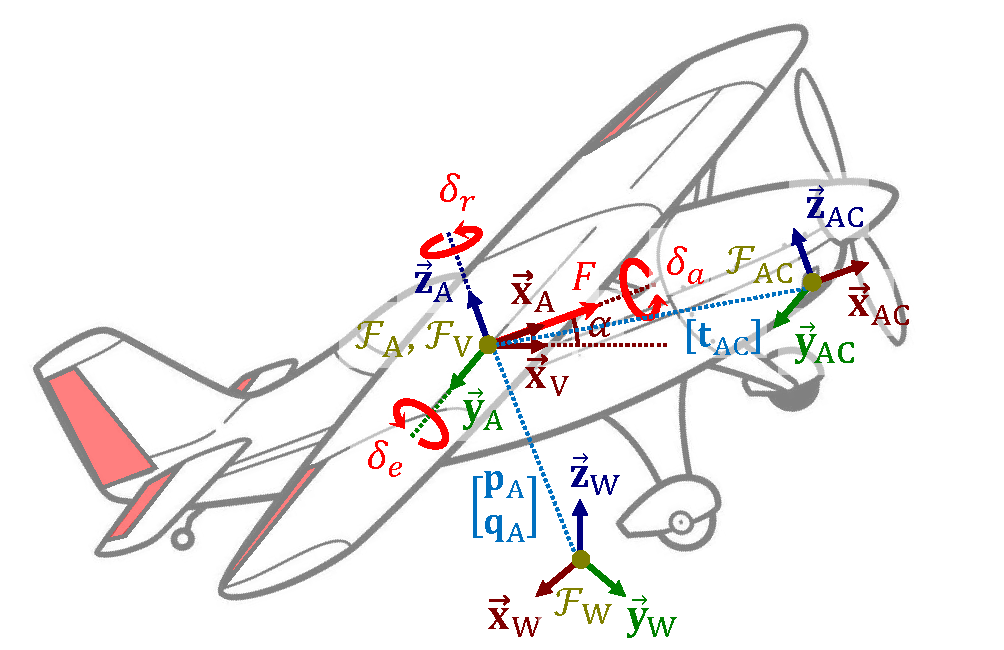
\includegraphics[width=0.9\columnwidth, trim={0 0 1cm 0}, clip]{plane.pdf}%
\caption{Fixed-wing aircraft shown with its reference frames, control inputs (in red) and output variables (in blue).}
\label{fig:plane}
\end{figure}
%%%%%%%%%%%%%%%%%%%%

Fixed-wing aircraft (in Fig.~\ref{fig:plane}) are underactuated dynamic systems. 
Let $\mathcal{F}_\text{A}$ be the aircraft's body frame. The aircraft's pose is given by its position $\mathbf p_\text{A} = \begin{bmatrix} x_\text{A} & y_\text{A} & z_\text{A} \end{bmatrix}^\top \in \mathbb{R}^3$ in $\mathcal F_\text{W}$ and a quaternion $\mathbf q_\text{A} \in \mathbb{H}_1$ mapping $\mathcal F_\text{A} \to \mathcal F_\text{W}$ with $\phi_\text{A}$, $\theta_\text{A}$ and $\psi_\text{A}$ being roll, pitch and yaw angles, respectively. 
Aircraft's linear and angular velocities in $\mathcal{F}_\text{A}$ are $\mathbf{v}_\text{A} \in \mathbb{R}^3$ and $\boldsymbol{\omega}_\text{A} \in \mathbb{R}^3$, respectively.
The aircraft's state is
%%%%%%%%%%%%%%%%%%%%
\begin{equation}
\mathbf{x}_\text{A} = \begin{bmatrix} \mathbf{p}_\text{A} & \mathbf{q}_\text{A} & \mathbf{v}_\text{A} & \boldsymbol{\omega}_\text{A} \end{bmatrix}^\top,
\label{eq:plane_x}
\end{equation}
%%%%%%%%%%%%%%%%%%%%
while the output is
%%%%%%%%%%%%%%%%%%%%
\begin{equation}
\mathbf{y}_\text{A} = \begin{bmatrix} \mathbf{p}_\text{A}^\top & \mathbf{q}_\text{A}^\top \end{bmatrix}.
\label{eq:plane_y}
\end{equation}
%%%%%%%%%%%%%%%%%%%%

Commonly, the control input to a fixed-wing aircraft is 
%%%%%%%%%%%%%%%%%%%%
\begin{equation}
\mathbf{u}_\text{A} = \begin{bmatrix} F & \delta_a & \delta_e & \delta_r \end{bmatrix}^\top,
\label{eq:plane_u}
\end{equation}
%%%%%%%%%%%%%%%%%%%%
where $F$ is the thrust generated by the engines, $\delta_a$, $\delta_e$, and $\delta_r$ are  aileron, elevator, and
rudder deflections.
Aerodynamic forces acting on a fixed-wing aircraft defined in the wind frame $\mathcal{F}_\text{V}$ are $\mathbf{f}_\text{aero} = \begin{bmatrix} -D & Y & L \end{bmatrix}^\top$, with $D \propto v^2$ is drag, $Y$ is side force, $L \propto v^2$ is lift, and $v$ is airspeed. The total force acting on the fixed-wing aircraft in $\mathcal{F}_\text{A}$ is $\mathbf{f}_\text{A} = \mathbf{R}(\alpha) \mathbf{f}_\text{aero} + \begin{bmatrix} F & 0 & 0 \end{bmatrix}^\top + \mathbf{R}\left(\mathbf{q}_\text{A}\right)^\top \begin{bmatrix} 0 & 0 & -g \end{bmatrix}^\top$, where $\alpha$ is the angle of attack, and $g$ is the gravitational constant.
The total torque acting on the fixed-wing aircraft in $\mathcal{F}_\text{A}$ is $\boldsymbol{\tau}_\text{A} = \mathbf{B}_\tau \begin{bmatrix} \delta_a & \delta_e & \delta_r \end{bmatrix}^\top$, where $\mathbf{B}_\tau$ is the control-effectiveness map.
Using the Newton-Euler equations, the kinematics and dynamics of a fixed-wing aircraft are:
%%%%%%%%%%%%%%%%%%%%
\begin{equation}
f_\text{A}:
\begin{cases}
\dot{\mathbf{p}}_\text{A} = \mathbf{R}\left(\mathbf{q}_\text{A}\right) \mathbf{v}_\text{A} \\
\dot{\mathbf{q}}_\text{A} = \frac{1}{2} \mathbf{G}\left(\mathbf{q}_\text{A}\right) \boldsymbol{\omega}_\text{A} \\
\dot{\mathbf{v}}_\text{A} = -\boldsymbol{\omega}_\text{A} \times \mathbf{v}_\text{A} + \frac{1}{m_\text{A}} \mathbf{f}_\text{A} \\
\dot{\boldsymbol{\omega}}_\text{A} = -\left(\mathbf{J}_\text{A}\right)^{-1} \boldsymbol{\omega}_\text{A} \times (\mathbf{J}_\text{A} \boldsymbol{\omega}_\text{A}) + \left(\mathbf{J}_\text{A}\right)^{-1} \boldsymbol{\tau}_\text{A}
\end{cases},
\label{eq:plane_dynamics}
\end{equation} 
%%%%%%%%%%%%%%%%%%%%
in which %$R\left(\mathbf{q}\right)$ is the rotation matrix from $\mathcal{F}_B$ to $\mathcal{F}_W$, % is $R\left(\mathbf{q}\right) = \begin{bmatrix} 1 - 2(q_y^2 + q_z^2) & 2(q_x q_y - q_w q_z) & 2(q_x q_z + q_w q_y) \\ 2(q_x q_y + q_w q_z) & 1 - 2(q_x^2 + q_z^2) & 2(q_y q_z - q_w q_x) \\ 2(q_x q_z - q_w q_y) & 2(q_y q_z + q_w q_x) & 1 - 2(q_x^2 + q_y^2) \end{bmatrix}$, 
$\mathbf{G}\left(\mathbf{q}\right) \in \mathbb{R}^{4 \times 3}$ % = \begin{bmatrix} -q_x & -q_y & -q_z \\ q_w & -q_z & q_y \\ q_z & q_w & -q_x \\ -q_y & q_x & q_w \end{bmatrix}$ 
is the quaternion kinematics matrix, $m_\text{A}$ is aircraft's mass, and $\mathbf{J}_\text{A} \in \mathbb{R}^{3 \times 3}$ is matrix of inertia.

%%%%%%%%%%%%%%%%%%%%%%%%%%%%%%%%%%%%%%%%%%%%%%%%%%%%%%%%%%%%%%%%%%%%%%%%%%%%%%%%
%%%%%%%%%%%%%%%%%%%%%%%%%%%%%%%%%%%%%%%%%%%%%%%%%%%%%%%%%%%%%%%%%%%%%%%%%%%%%%%%
\subsection{Multicopter with 2-Axis Gimbal Dynamics}

%%%%%%%%%%%%%%%%%%%%
\begin{figure}[!b]
\centering
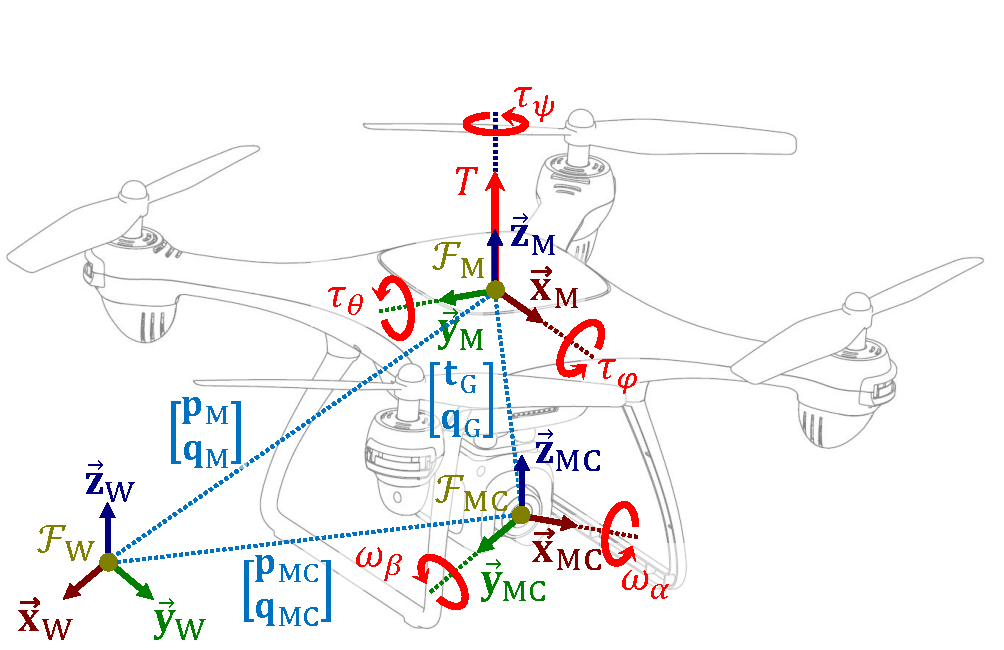
\includegraphics[width=0.9\columnwidth, trim={0 0 0 1cm}, clip]{quad.pdf}%
\caption{Multicopter with two-axis gimbal shown with its reference frames, control inputs (in red) and output variables (in blue).}
\label{fig:quadcopter}
\end{figure}
%%%%%%%%%%%%%%%%%%%%

Multicopters (in Fig.~\ref{fig:quadcopter}) are also underactuated dynamic systems. 
Let $\mathcal{F}_\text{M}$ be the multicopter's body frame. The multicopter's pose is given by its position $\mathbf p_\text{M} = \begin{bmatrix} x_\text{M} & y_\text{M} & z_\text{M} \end{bmatrix}^\top \in \mathbb{R}^3$ in $\mathcal F_\text{W}$ and a quaternion $\mathbf q_\text{M} \in \mathbb{H}_1$ mapping $\mathcal F_\text{M} \to \mathcal F_\text{W}$ with $\phi_\text{M}$, $\theta_\text{M}$ and $\psi_\text{M}$ being roll, pitch and yaw angles, respectively. 
Multicopter's linear and angular velocities in $\mathcal{F}_\text{M}$ are $\mathbf{v}_\text{M} \in \mathbb{R}^3$ and $\boldsymbol{\omega}_\text{M} \in \mathbb{R}^3$, respectively.
The multicopter is equipped with a camera mounted on a 2-axis roll-pitch gimbal with joint angles $\phi_\text{G}$ and $\theta_\text{G}$ and quaternion $\mathbf{q}_\text{MC} = \mathbf{q}_x(\phi_\text{G}) \otimes \mathbf{q}_y(\theta_\text{G}) \in \mathbb{H}_1$, which maps from the multicopter's camera frame $\mathcal{F}_\text{MC}$ to $\mathcal{F}_\text{M}$. Let the camera lever arm in $\mathcal{F}_\text{M}$ be $\mathbf{t}_\text{G} \in \mathbb{R}^3$.
The state of a multicopter with a two-axis gimbal is 
%%%%%%%%%%%%%%%%%%%%
\begin{equation}
\mathbf{x}_\text{M} = \begin{bmatrix} \mathbf{p}_\text{M} & \mathbf{q}_\text{M} & \mathbf{v}_\text{M} & \boldsymbol{\omega}_\text{M} & \mathbf{q}_\text{G} \end{bmatrix}^\top,
\label{eq:quad_x}
\end{equation}
%%%%%%%%%%%%%%%%%%%%
while the output is the camera's pose:
%%%%%%%%%%%%%%%%%%%%
\begin{equation}
\mathbf{y}_\text{MC} = \begin{bmatrix} \mathbf{p}_\text{M}^\top + \left( R\left(\mathbf{q}_\text{M}\right) \mathbf{t}_\text{G} \right)^\top & \left( \mathbf{q}_\text{M} \otimes \mathbf{q}_\text{G} \right)^\top \end{bmatrix}.
\label{eq:gimbal_y}
\end{equation}
%%%%%%%%%%%%%%%%%%%%

Commonly, the control input to a multicopter is 
%%%%%%%%%%%%%%%%%%%%
\begin{equation}
\mathbf{u}_\text{M} = \begin{bmatrix} T & \tau_\phi & \tau_\theta & \tau_\psi \end{bmatrix}^\top,
\label{eq:quad_u}
\end{equation}
%%%%%%%%%%%%%%%%%%%%
where $T$ is total thrust, $\tau_\phi$, $\tau_\theta$, and $\tau_\psi$ are torques around $x$-, $y$- and $z$-axes, respectively. Control inputs to the gimbal are
%%%%%%%%%%%%%%%%%%%%
\begin{equation}
\mathbf{u}_\text{G} = \begin{bmatrix} \dot\theta_\text{G} & \dot\psi_\text{G} \end{bmatrix}^\top.
\label{eq:gimbal_u}
\end{equation}
%%%%%%%%%%%%%%%%%%%%
%where $\dot\theta_\text{G}$ and $\dot\psi_\text{G}$ are gimbal's roll and pitch rates, respectively.
The total force acting on the multicopter in $\mathcal{F}_\text{M}$ is $\mathbf{f}_\text{M} = \begin{bmatrix} 0 & 0 & T \end{bmatrix}^\top + \mathbf{R}\left(\mathbf{q}_\text{M}\right)^\top \begin{bmatrix} 0 & 0 & -g \end{bmatrix}^\top$; while the total torque in $\mathcal{F}_\text{M}$ is $\boldsymbol{\tau}_\text{M} = \begin{bmatrix} \tau_\phi & \tau_\theta & \tau_\psi \end{bmatrix}^\top$.
So, the kinematics and dynamics of a multicopter with a gimbal are:
%%%%%%%%%%%%%%%%%%%%
\begin{equation}
f_\text{M}:
\begin{cases}
\dot{\mathbf{p}}_\text{M} = \mathbf{R}\left(\mathbf{q}_\text{M}\right) \mathbf{v}_\text{M} \\
\dot{\mathbf{q}}_\text{M} = \frac{1}{2} \mathbf{G}\left(\mathbf{q}_\text{M}\right) \boldsymbol{\omega}_\text{M} \\
\dot{\mathbf{v}}_\text{M} = -\boldsymbol{\omega}_\text{M} \times \mathbf{v}_\text{M} + \frac{1}{m_\text{M}} \mathbf{f}_\text{M} \\
\dot{\boldsymbol{\omega}}_\text{M} = -\left(\mathbf{J}_\text{M}\right)^{-1} \boldsymbol{\omega}_\text{M} \times (\mathbf{J}_\text{M} \boldsymbol{\omega}_\text{M}) + \left(\mathbf{J}_\text{M}\right)^{-1} \boldsymbol{\tau}_\text{M} \\
\dot{\mathbf{q}}_\text{MC} = \frac{1}{2} \mathbf{G}\left(\mathbf{q}_\text{MC}\right) \mathbf{u}_\text{G}
\end{cases},
\label{eq:quad_dynamics}
\end{equation} 
%%%%%%%%%%%%%%%%%%%%
in which $m_\text{M}$ is the mass of multicopter with gimbal, and $\mathbf{J}_\text{M} \in \mathbb{R}^{3 \times 3}$ is matrix of inertia.

%%%%%%%%%%%%%%%%%%%%%%%%%%%%%%%%%%%%%%%%%%%%%%%%%%%%%%%%%%%%%%%%%%%%%%%%%%%%%%%%
%%%%%%%%%%%%%%%%%%%%%%%%%%%%%%%%%%%%%%%%%%%%%%%%%%%%%%%%%%%%%%%%%%%%%%%%%%%%%%%%
%%%%%%%%%%%%%%%%%%%%%%%%%%%%%%%%%%%%%%%%%%%%%%%%%%%%%%%%%%%%%%%%%%%%%%%%%%%%%%%%
\section{Camera-Pose Controllability and Mimicry on $SE(3)$}
\label{sec:proof}

%%%%%%%%%%%%%%%%%%%%%%%%%%%%%%%%%%%%%%%%%%%%%%%%%%%%%%%%%%%%%%%%%%%%%%%%%%%%%%%%
Assume the fixed-wing carries a camera that is body-aligned and located at a fixed lever arm $\mathbf{t}_\text{AC} \in \mathbb{R}^3$ expressed in $\mathcal{F}_\text{A}$.
Then, the fixed-wing camera pose is
%%%%%%%%%%%%%%%%%%%%
\begin{equation}
\mathbf{y}_\text{AC} = \begin{bmatrix} \mathbf{p}_\text{AC}^\top & \mathbf{q}_\text{AC}^\top \end{bmatrix}
= \begin{bmatrix} \big( \mathbf{p}_\text{A} + \mathbf{R}\left( \mathbf{q}_\text{A} \right) \mathbf{t}_\text{AC} \big)^\top & \mathbf{q}_\text{A}^\top \end{bmatrix}.
\label{eq:plane_camera_pose}
\end{equation}
%%%%%%%%%%%%%%%%%%%%

% \begin{theorem}[Camera-pose mimicry]
% Under assumptions~\ref{ass:authority} and \ref{ass:non_singularity}, there exist multicopter inputs $\mathbf{u}_\text{M}$ and gimbal rates $\mathbf{u}_\text{G}$ such that
% %%%%%%%%%%%%%%%%%%%%
% \begin{equation}
% \label{eq:goal_equal}
% \mathbf{y}_\text{MC}(t) \equiv \mathbf{y}_\text{AC}(t) \quad \forall t.
% \end{equation}
% %%%%%%%%%%%%%%%%%%%%
% \end{theorem}

% Our goal is to realize $\mathbf{y}^{C}(t)\equiv\mathbf{y}^{A\!\to C}(t)$ along any \emph{feasible} trajectory.

We expose (i) a translational ``virtual'' input $\,\mathbf{a}_\text{MC} \in \mathbb{R}^3$ realized by the standard $SE(3)$ inner loop (third line of~\eqref{eq:quad_dynamics}), and (ii) rotational inputs $\dot{\boldsymbol{\Theta}}_\text{MC} = \begin{bmatrix} \dot\phi_\text{G} & \dot\theta_\text{G} & \dot\psi_\text{M} \end{bmatrix}^\top$ consisting of gimbal roll and pitch rates and the multicopter’s free body yaw rate around $\vec{\mathbf{z}}_\text{M}$, which does not alter the thrust direction.

From \eqref{eq:gimbal_y}, the position of the multicopter's camera in the $\mathcal{F}_\text{W}$ is 
%%%%%%%%%%%%%%%%%%%%
\begin{equation}\mathbf{p}_\text{MC} = \mathbf{p}_\text{M} + \mathbf{R}(\mathbf{q}_\text{M}) \mathbf{t}_\text{G},\
\label{eq:p_mc}
\end{equation}
%%%%%%%%%%%%%%%%%%%%
while the rotation is 
%%%%%%%%%%%%%%%%%%%%
\begin{equation}
\mathbf{q}_\text{MC} = \mathbf{q}_\text{M} \otimes \mathbf{q}_\text{G}. 
\label{eq:q_mc}
\end{equation}
%%%%%%%%%%%%%%%%%%%%
Then, by \eqref{eq:p_mc}
%%%%%%%%%%%%%%%%%%%%
\begin{equation}
\ddot{\mathbf{p}}_\text{MC} = \mathbf{a}_\text{M} + \boldsymbol{\Delta}(\mathbf{p}_\text{MC}, \mathbf{q}_\text{M}, \boldsymbol{\omega}_\text{M}, \dot{\boldsymbol{\omega}}_\text{M}),
\label{eq:pc_ddot}
\end{equation}
%%%%%%%%%%%%%%%%%%%%
where $\boldsymbol\Delta(\mathbf{p}_\text{MC}, \mathbf{q}_\text{M}, \boldsymbol{\omega}_\text{M}, \dot{\boldsymbol{\omega}}_\text{M})$ collects the known lever-arm coupling terms, and by \eqref{eq:q_mc}
%%%%%%%%%%%%%%%%%%%%
\begin{equation}
\dot{\mathbf{q}}_\text{MC} = \frac{1}{2} \mathbf{G}(\mathbf{q}_\text{MC}) \boldsymbol{\omega}_\text{MC},
\label{eq:qc_dot}
\end{equation}
%%%%%%%%%%%%%%%%%%%%
where $\boldsymbol{\omega}_\text{MC} = \mathbf{S}(\phi_\text{G}, \theta_\text{G}) \dot{\boldsymbol{\Theta}}_\text{MC}$ with the input-twist matrix
\begin{equation}
\mathbf{S}(\phi,\theta)=
\begin{bmatrix}
1 & 0 & -\sin\theta\cos\phi\\
0 & 1 & -\sin\phi\\
0 & 0 & \ \cos\theta\cos\phi
\end{bmatrix},
\label{eq:S_matrix}
\end{equation}
whose determinant is 
%%%%%%%%%%%%%%%%%%%%
\begin{equation}
\det \mathbf{S}(\phi,\theta)=\cos\theta\,\cos\phi.
\label{eq:S_determinant}
\end{equation}
%%%%%%%%%%%%%%%%%%%%

\begin{remark}
Singularities for a 2-axis gimbal occur at $\cos\phi_\text{G}\cos\theta_\text{G} = 0$.
\end{remark}

\begin{assumption}[Non-Singularity]
\label{ass:non_singularity}
The multicopter gimbal attitude stays away from the singular set: $\phi_\text{G} \neq \pm \frac{\pi}{2} \land \theta_\text{G} \neq \pm \frac{\pi}{2}$.
\end{assumption}

\begin{remark}
This assumption can be relaxed by using a planner which will avoid the singular set.
\end{remark}

%%%%%%%%%%%%%%%%%%%%%%%%%%%%%%%%%%%%%%%%%%%%%%%%%%%%%%%%%%%%%%%%%%%%%%%%%%%%%%%%
%%%%%%%%%%%%%%%%%%%%%%%%%%%%%%%%%%%%%%%%%%%%%%%%%%%%%%%%%%%%%%%%%%%%%%%%%%%%%%%%
\subsection{Output Full Actuation \& STLC on $SE(3)$}
\label{ssec:controllability}

Consider the block-triangular Jacobian from inputs to camera acceleration and twist:
%%%%%%%%%%%%%%%%%%%%
\begin{equation}
\label{eq:J_block}
\begin{bmatrix} \ddot{\mathbf{p}}_\text{MC} \\ \boldsymbol{\omega}_\text{MC} \end{bmatrix} = 
\underbrace{\begin{bmatrix} \mathbf{I}_3 & \mathbf{0} \\ \mathbf{0} & \mathbf{S}(\phi_\text{G},\theta_\text{G})\end{bmatrix}}_{\mathbf{J}} \begin{bmatrix} \mathbf{a}_\text{MC} \\ \dot{\boldsymbol{\Theta}}_\text{MC} \end{bmatrix} + \begin{bmatrix} \boldsymbol\Delta \\ \mathbf{0} \end{bmatrix}.
\end{equation}
%%%%%%%%%%%%%%%%%%%%

\paragraph{Translational rank}
Thrust vectoring yields $\mathbf{a}_\text{MC} = -g \mathbf{e}_3 + \frac{T}{m_\text{M}} \mathbf{b}_3$; variations $\delta \mathbf{a}_\text{MC} = \frac{\delta T}{m_\text{M}} \mathbf{b}_3 + \frac{T}{m_\text{M}} \delta \mathbf{b}_3$ span $\mathbb{R}^3$. Hence, $\mathbf{a}_\text{MC} \mapsto \ddot{\mathbf{p}}_\text{MC}$ is locally surjective.

\paragraph{Rotational rank}
By \eqref{eq:S_determinant}, $\mathrm{rank}(\mathbf{S}) = 3$, whenever $\cos\phi_\text{G}\cos\theta_\text{G} \neq 0$.

Therefore, $\mathrm{rank}(\mathbf{J}) = 6$ almost everywhere, and the camera pose is \emph{output fully actuated} and \emph{small-time locally controllable}~(STLC) on $SE(3)$. 

\begin{remark}
With a 3-axis gimbal ($\mathbf{S} \equiv \mathbf{I}_3$), the result holds globally. 
\end{remark}

%%%%%%%%%%%%%%%%%%%%%%%%%%%%%%%%%%%%%%%%%%%%%%%%%%%%%%%%%%%%%%%%%%%%%%%%%%%%%%%%
%%%%%%%%%%%%%%%%%%%%%%%%%%%%%%%%%%%%%%%%%%%%%%%%%%%%%%%%%%%%%%%%%%%%%%%%%%%%%%%%
\subsection{Camera-Pose Mimicry}
\label{ssec:mimicry}

Now we show that multicopter and gimbal control inputs exist so that 
%%%%%%%%%%%%%%%%%%%%
\begin{equation}
\mathbf{y}_\text{MC}(t) \equiv \mathbf{y}_\text{AC}(t) \quad \forall t.
\end{equation}
%%%%%%%%%%%%%%%%%%%%

\begin{assumption}[Authority]
\label{ass:authority}
Thrust and torque of the multicopter, as well as gimbal angle/rate limits, are not violated along the trajectories of interest.
\end{assumption}

\paragraph{Position matching}
Equality of camera positions, $\mathbf{p}_\text{M} + \mathbf{R}(\mathbf{q}_\text{M})\mathbf{t}_\text{G} = \mathbf{p}_\text{A} + \mathbf{R}(\mathbf{q}_\text{A})\mathbf{t}_\text{AC}$, is realised by commanding the multicopter position to the lever-arm-compensated target
%%%%%%%%%%%%%%%%%%%%
\begin{equation}
\label{eq:pos_cmd_combined}
\mathbf{p}_\text{M} = \mathbf{p}_\text{A} + \mathbf{R}(\mathbf{q}_\text{A})\mathbf{t}_\text{AC} - \mathbf{R}(\mathbf{q}_\text{M})\mathbf{t}_\text{G}.
\end{equation}
%%%%%%%%%%%%%%%%%%%%
Taking two derivatives gives the desired multicopter's acceleration
%%%%%%%%%%%%%%%%%%%%
\begin{equation}
\mathbf{a}_\text{M} = \ddot{\mathbf{p}}_\text{A} + \frac{d^2 \mathbf{R}(\mathbf{q}_\text{A})}{dt^2} \mathbf{t}_\text{AC} - \frac{d^2 \mathbf{R}(\mathbf{q}_\text{M})}{dt^2} \mathbf{t}_\text{G},
\end{equation}
%%%%%%%%%%%%%%%%%%%%
which the $SE(3)$ inner loop (third line of \eqref{eq:quad_dynamics}) can track so that $\mathbf{p}_\text{M} + \mathbf{R}(\mathbf{q}_\text{M})\mathbf{t}_\text{G} \rightarrow \mathbf{p}_\text{A} + \mathbf{R}(\mathbf{q}_\text{A})\mathbf{t}_\text{AC}$.

\paragraph{Orientation matching}
We require $\mathbf{q}_\text{M} \otimes \mathbf{q}_\text{G} = \mathbf{q}_\text{A}$. Decompose the multicopter attitude into free yaw and tilt:
%%%%%%%%%%%%%%%%%%%%
\begin{equation}
\label{eq:q_split_combined}
\mathbf{q}_\text{M} = \mathbf{q}_z(\psi_\text{M}) \otimes \mathbf{q}_\text{tilt},
\end{equation}
%%%%%%%%%%%%%%%%%%%%
where $\mathbf{q}_\text{tilt}$ sets the thrust direction dictated by $\mathbf{a}_\text{M}$, and $\psi_\text{M}$ is the free yaw about $\vec{\mathbf{z}}_\text{M}$.
Define relative camera quaternion
%%%%%%%%%%%%%%%%%%%%
\begin{equation}
\label{eq:q_rel_combined}
\mathbf{q}_\text{rel} = \bar{\mathbf{q}}_\text{M} \otimes \mathbf{q}_\text{A} = \bar{\mathbf{q}}_\text{tilt} \otimes \mathbf{q}_z(-\psi_\text{M}) \otimes \mathbf{q}_\text{A}.
\end{equation}
%%%%%%%%%%%%%%%%%%%%
To cancel the yaw, choose
%%%%%%%%%%%%%%%%%%%%
\begin{equation}
\label{eq:yaw_sched_combined}
\bar{\psi}_\text{M} = \mathrm{yaw}\left( \bar{\mathbf{q}}_\text{tilt} \otimes \mathbf{q}_\text{A} \right).
\end{equation}
%%%%%%%%%%%%%%%%%%%%
Then, $\mathbf{q}_\text{rel}$ has zero yaw and, therefore, lies in the roll-pitch submanifold. Hence, there exist $(\phi_\text{G}, \theta_\text{G})$ such that
%%%%%%%%%%%%%%%%%%%%
\begin{equation}
\label{eq:qG_choice_combined}
\mathbf{q}_\text{G} = \mathbf{q}_x(\phi_\text{G}) \otimes \mathbf{q}_y(\theta_\text{G}) = \mathbf{q}_\text{rel}.
\end{equation}
%%%%%%%%%%%%%%%%%%%%
This yields $\mathbf{q}_\text{M} \otimes \mathbf{q}_\text{G} = \mathbf{q}_\text{A}$, so camera orientations match exactly.

Under Assumptions~\ref{ass:non_singularity} and \ref{ass:authority}, the multicopter with a \mbox{2-axis} gimbal is output fully actuated and STLC on $SE(3)$ for the camera pose, and control inputs exist which realise $\mathbf{y}_\text{MC}(t) \equiv \mathbf{y}_\text{AC}(t)$ for any feasible fixed-wing camera trajectory. With identical intrinsics, the rendered image streams are indistinguishable to the viewer.

%%%%%%%%%%%%%%%%%%%%%%%%%%%%%%%%%%%%%%%%%%%%%%%%%%%%%%%%%%%%%%%%%%%%%%%%%%%%%%%%
%%%%%%%%%%%%%%%%%%%%%%%%%%%%%%%%%%%%%%%%%%%%%%%%%%%%%%%%%%%%%%%%%%%%%%%%%%%%%%%%
%%%%%%%%%%%%%%%%%%%%%%%%%%%%%%%%%%%%%%%%%%%%%%%%%%%%%%%%%%%%%%%%%%%%%%%%%%%%%%%%
\section{Proposed Method}
\label{sec:method}

Given the fixed-wing camera trajectory $\mathbf{y}_\text{AC}(t)$ in~\eqref{eq:plane_camera_pose}, we want to compute multicopter and gimbal inputs, 
%%%%%%%%%%%%%%%%%%%%
\begin{equation}
\mathbf{u}_\text{MC} = \begin{bmatrix} \mathbf{u}_\text{M} \\ \mathbf{u}_\text{G} \end{bmatrix},
\label{eq:u_MC}
\end{equation}
%%%%%%%%%%%%%%%%%%%%
such that the multicopter camera pose $\mathbf{y}_\text{MC}(t)$ in~\eqref{eq:gimbal_y} satisfies $\mathbf{y}_\text{MC}(t) \equiv \mathbf{y}_\text{AC}(t) \quad \forall t$.

To enable multicopter tracking aggressive manoeuvres, non-linear control techniques must be used. Dynamic feedback linearization~(DFL) could be designed to achieve better convergence and robustness. Through a change of variables, DFL transforms a nonlinear system into an equivalent linear, controllable and observable one.
Given a non-linear system
%%%%%%%%%%%%%%%%%
\begin{equation}
\begin{cases}
\dot{\mathbf{x}} = f(\mathbf{x}) + g(\mathbf{x}) \mathbf{u} \\
\mathbf{y} = h(\mathbf{x}),
\end{cases}
\label{eq:nonlinear_system}
\end{equation}
%%%%%%%%%%%%%%%%%
where $\mathbf{x}$ is the system state, $\mathbf{u}$ is the system input, $\mathbf{y}$ is the system output, $f(\mathbf{x})$, $g(\mathbf{x})$ and $h(\mathbf{x})$ are vector fields in $\mathbb{R}^n$. The task of feedback linearization is to identify a static state feedback control law of the following form:
%%%%%%%%%%%%%%%%%
\begin{equation}
\mathbf{u} = \alpha(\mathbf{x}) + \beta(\mathbf{x}) \mathbf{v},
\label{eq:feedback_control}
\end{equation}
%%%%%%%%%%%%%%%%%
where $\mathbf{v}$ is an new control input, $\alpha(\mathbf{x})$ and $\beta(\mathbf{x})$ are smooth functions defined in a neighbourhood of some point $\mathbf{x}_0 \in  \mathbb{R}^n$ and $\beta(\mathbf{x}_0) \neq 0$, such that the closed-loop system composed of (\ref{eq:nonlinear_system}) and (\ref{eq:feedback_control}) behaves as a linear and completely accessible system.
For system (\ref{eq:nonlinear_system}), let $N_\text{I}$ be the number of inputs, $N_\text{O}$ be the number of outputs, $\mathbf{r} = \begin{bmatrix}r_1 & \cdots & r_{N_\text{O}}\end{bmatrix}$ be the vector relative degree. Then, let's define
%%%%%%%%%%%%%%%%%
\begin{equation}
\Delta(\mathbf{x}) = \begin{bmatrix}
L_{g_1} L^{r_1 - 1}_f h_1(\mathbf{x}) & \cdots & L_{g_{N_\text{I}}} L^{r_1 - 1}_f h_1(\mathbf{x}) \\
\vdots & \ddots & \vdots \\
L_{g_1} L^{r_{N_\text{O}} - 1}_f h_{N_\text{O}}(\mathbf{x}) & \cdots & L_{g_{N_\text{I}}} L^{r_{N_\text{O}} - 1}_f h_{N_\text{O}}(\mathbf{x})
\end{bmatrix}
\label{eq:delta}
\end{equation}
%%%%%%%%%%%%%%%%%
and
%%%%%%%%%%%%%%%%%
\begin{equation}
b(\mathbf{x}) = \begin{bmatrix}L^{r_1}_f h_1(\mathbf{x}) & \cdots & L^{r_{N_\text{O}}}_f h_{N_\text{O}}(\mathbf{x})\end{bmatrix}^T,
\label{eq:b}
\end{equation}
%%%%%%%%%%%%%%%%%
where $L^r_f h$ denotes the $r$-th Lie derivative of the function $h$ with respect to the vector field $f$.
The main result about the input-output decoupling problem is that this problem is solvable if and only if the matrix $\Delta(\mathbf{x})$ is non-singular. In that case, the static state feedback (\ref{eq:feedback_control}) with
%%%%%%%%%%%%%%%%%
\begin{equation}
\begin{cases}
\alpha(\mathbf{x}) = -\left( \Delta(\mathbf{x}) \right)^{-1} b(\mathbf{x}) \\
\beta(\mathbf{x}) = \left( \Delta(\mathbf{x}) \right)^{-1}
\end{cases}
\label{eq:alpha_beta}
\end{equation}
%%%%%%%%%%%%%%%%%
renders the closed-loop system linear and decoupled from an input-output point of view.

To feedback linearize a system, the necessary and sufficient condition for the solvability of the state space exact linearization problem is \cite{Isidori1986CDC}:
%%%%%%%%%%%%%%%%%%%%
\begin{equation}
\sum_{i = 1}^{N_\text{O}}{r_i} = N,
\label{eq:condition}
\end{equation}
%%%%%%%%%%%%%%%%%%%%
where $N$ is the system's rank.

%%%%%%%%%%%%%%%%%
\tikzstyle{int}=[draw, align=center, fill=blue!0, minimum size=2em, text width=1cm]
\tikzstyle{sum}=[draw, fill=blue!0, shape=circle, inner sep=0.3pt]
\begin{figure}[!b]
\centering
    \resizebox{0.99\columnwidth}{!}{
    \begin{tikzpicture}[node distance=1cm, auto, >=latex', line width=0.5mm]
        \node[int, text width=2cm, minimum height=1cm, fill=red!20](f_A){$f_\text{A}(\mathbf{x}_\text{A})$};
        |%\node[int, below=1cm of f_A, text width=2cm, minimum height=1cm, fill=blue!20](f_A1){$f_\text{A}(\mathbf{x}_\text{A})$};
        \node[int, below right=0.5cm and 0cm of f_A, text width=2cm, minimum height=1cm, fill=blue!20](f_M1){$\hat{f}_\text{M}^{-1}(\hat{\mathbf{x}}_\text{M})$};
        \node[int, right=1cm of f_M1, text width=2cm, minimum height=1cm, fill=blue!20](f_M){$\hat{f}_\text{M}(\hat{\mathbf{x}}_\text{M})$};
   
        \draw[->] ($(f_A.west) + (-1cm, 0)$) -- node{$\mathbf{u}_\text{A}$} (f_A.west);
        \draw[->] (f_A.east) -- node{$\mathbf{y}_\text{AC}$} ++(1cm, 0);
        %\draw[->] ($(f_A.west) + (-0.5cm, 0)$) |- (f_A1.west);
        \draw[->] (f_A.south) |- node[pos=0.2]{$\mathbf{v}_\text{MC}$} (f_M1.west);
        \draw[->] (f_M1.east) -- node{$\hat{\mathbf{u}}_\text{MC}$} (f_M.west);
        \draw[->] (f_M.east) -- node{$\mathbf{y}_\text{MC}$} ++(1cm, 0);
        \draw[->] (f_M.south) -- node{$\hat{\mathbf{x}}_\text{M}$} ($(f_M.south) + (0, -0.5cm)$) -| (f_M1.south);
    \end{tikzpicture}}
\caption{Overview of the proposed framework.}
\label{fig:framework}
\end{figure}
%%%%%%%%%%%%%%%%%

For the system~(\ref{eq:quad_dynamics}), it can be shown that $\mathbf{r} = \begin{bmatrix}2 & 2 & 2 & 1 & 1 & 1\end{bmatrix}$, and $N = 14$ ~\cite{sarabakha2025data}. Since, $\sum_{i = 1}^{6}{r_i} = 9 \neq 14$, the condition~(\ref{eq:condition}) is not satisfied. Therefore, the input-output decoupling problem is not solvable for the system~(\ref{eq:quad_dynamics}) by means of a static state feedback control law. In fact, $\Delta(\mathbf{x}_\text{M})$ is singular for any $\mathbf{x}_\text{M}$ and is not invertible. So, the system (\ref{eq:quad_dynamics}) can not be transformed into an equivalent linear and controllable one by static state feedback. This is due to the fact that $\mathbf{a}_\text{M}$ is affected only by thrust $T$ and not by other control inputs. In order to get $\Delta(\mathbf{x})$ non-singular, the appearance of $T$ should be delayed to higher order derivatives of $\mathbf{a}_\text{M}$. This can be achieved by a dynamic compensator which incorporates an additional set of state variables $\boldsymbol{\chi}$ to achieve higher relative degrees~\cite{Mistler2001ROMAN}.
By setting $T$ equal to the output of an auxiliary dynamic system driven by a new reference input $\hat{T}$. The simplest way in which this result can be achieved is to set this auxiliary dynamic system equal to a double integrator. In this case, $\boldsymbol{\chi} = \begin{bmatrix} \chi_1 & \chi_2 \end{bmatrix}^\top$. So, $T$ is set equal to the output of a double integrator driven by $\ddot{T}$. The other input variables in~\eqref{eq:u_MC} are unchanged.
Now, $T$ is not any-more an input for the system~\eqref{eq:quad_dynamics}, but becomes the internal state for the new dynamical system
%%%%%%%%%%%%%%%%%%%%
\begin{equation}
\hat{f}_\text{M}:
\begin{cases}
\dot{\mathbf{p}}_\text{M} = \mathbf{R}\left(\mathbf{q}_\text{M}\right) \mathbf{v}_\text{M} \\
\dot{\mathbf{q}}_\text{M} = \frac{1}{2} \mathbf{G}\left(\mathbf{q}_\text{M}\right) \boldsymbol{\omega}_\text{M} \\
\dot{\mathbf{v}}_\text{M} = -\boldsymbol{\omega}_\text{M} \times \mathbf{v}_\text{M} + \frac{1}{m_\text{M}} \begin{bmatrix} 0 & 0 & \chi \end{bmatrix}^\top \\
\dot{\boldsymbol{\omega}}_\text{M} = -\left(\mathbf{J}_\text{M}\right)^{-1} \boldsymbol{\omega}_\text{M} \times (\mathbf{J}_\text{M} \boldsymbol{\omega}_\text{M}) + \left(\mathbf{J}_\text{M}\right)^{-1} \boldsymbol{\tau}_\text{M} \\
\dot{\mathbf{q}}_\text{MC} = \frac{1}{2} \mathbf{G}\left(\mathbf{q}_\text{MC}\right) \mathbf{u}_\text{G} \\
\ddot{\chi} = \ddot{T}
\end{cases}.
\label{eq:new_quad_dynamics}
\end{equation} 
%%%%%%%%%%%%%%%%%%%%
The new control inputs to the system~\eqref{eq:new_quad_dynamics} are 
%%%%%%%%%%%%%%%%%%%%
\begin{equation}
\hat{\mathbf{u}}_\text{MC} = \begin{bmatrix}\ddot{T} & \tau_{\phi} & \tau_{\theta} & \tau_{\psi} & \dot\theta_\text{G} & \dot\psi_\text{G} \end{bmatrix}^\top.
\end{equation}
%%%%%%%%%%%%%%%%%%%%
The input-output decoupling problem is solvable for the system (\ref{eq:quad_dynamics}) by means of a dynamic feedback control law, if it is solvable via static feedback for the extended system (\ref{eq:new_quad_dynamics}). Since the extended system has $\hat{\mathbf{r}} = \begin{bmatrix} 4 & 4 & 4 & 2 & 1 & 1 \end{bmatrix}$ and $\hat{N} = 16$, the condition~\eqref{eq:condition} is satisfied. Thus, the input-output decoupling problem is solvable for the system (\ref{eq:new_quad_dynamics}) by means of a dynamic feedback control law as in~\eqref{eq:feedback_control}:
%%%%%%%%%%%%%%%%%%%%
\begin{equation}
\hat{\mathbf{u}}_\text{MC} = \alpha(\hat{\mathbf{x}}_\text{MC}) + \beta(\hat{\mathbf{x}}_\text{MC}) \mathbf{v}_\text{MC},
\label{eq:feedback_control_extended}
\end{equation}
where $\alpha(\hat{\mathbf{x}}_\text{MC})$ and $\beta(\hat{\mathbf{x}}_\text{MC})$ are computed using~\eqref{eq:alpha_beta}, and
%%%%%%%%%%%%%%%%%%%%
\begin{equation}
\mathbf{v}_\text{MC} = \begin{bmatrix} \mathbf{p}_\text{AC}^\top & \dot{\mathbf{p}}_\text{AC}^\top & \ddot{\mathbf{p}}_\text{AC}^\top & \dddot{\mathbf{p}}_\text{AC}^\top & \ddddot{\mathbf{p}}_\text{AC}^\top & \mathbf{q}_\text{A}^\top & \dot{\mathbf{q}}_\text{A}^\top & \ddot{\mathbf{q}}_\text{A}^\top \end{bmatrix}.
\end{equation}
An overview of the proposed framework is shown in Fig. \ref{fig:framework}.
%%%%%%%%%%%%%%%%%%%%

%%%%%%%%%%%%%%%%%%%%%%%%%%%%%%%%%%%%%%%%%%%%%%%%%%%%%%%%%%%%%%%%%%%%%%%%%%%%%%%%
%%%%%%%%%%%%%%%%%%%%%%%%%%%%%%%%%%%%%%%%%%%%%%%%%%%%%%%%%%%%%%%%%%%%%%%%%%%%%%%%
%%%%%%%%%%%%%%%%%%%%%%%%%%%%%%%%%%%%%%%%%%%%%%%%%%%%%%%%%%%%%%%%%%%%%%%%%%%%%%%%
%The five aerobatic maneuvers in the experimental task: (1) loop,(2) left slow roll, (3) inverted flight (½ left roll, 10 seconds inverted, ½ left roll),(4) Immelmann (½ loop, ½ left roll), and (5) Split-S (½ left roll, ½ loop)
% https://www.researchgate.net/profile/Jan-Roessingh/publication/228651624/figure/fig5/AS:668347255504914@1536357811713/The-five-aerobatic-maneuvers-in-the-experimental-task-1-loop-2-left-slow-roll-3.png
%Acrobatic maneuvers %\cite{roessingh2005transfer}.
% \subsection{Trajectory 3: Left Roll}



% \subsection{Trajectory 4: Inverted Flight}



% \subsection{Trajectory 5: Immelmann Turn}



% \subsection{Trajectory 6: Split-S}
\input{results}



%%%%%%%%%%%%%%%%%%%%%%%%%%%%%%%%%%%%%%%%%%%%%%%%%%%%%%%%%%%%%%%%%%%%%%%%%%%%%%%%
%%%%%%%%%%%%%%%%%%%%%%%%%%%%%%%%%%%%%%%%%%%%%%%%%%%%%%%%%%%%%%%%%%%%%%%%%%%%%%%%
%%%%%%%%%%%%%%%%%%%%%%%%%%%%%%%%%%%%%%%%%%%%%%%%%%%%%%%%%%%%%%%%%%%%%%%%%%%%%%%%
\section{Conclusions and Future Work}
\label{sec:conclusions}



This work has designed and validated a control framework for physical-to-physical emulation, demonstrating that a multicopter equipped with a two-axis gimbal can dynamically replicate the camera viewpoint and flight dynamics of a fixed-wing aircraft. Our approach, based on DFL, provides a practical method for achieving high-fidelity mimicry of a primary system's key observables. This capability enables algorithm validation and operator training in real-world conditions at a negligible cost and with significantly reduced operational risk compared to deploying the high-value fixed-wing planes. Furthermore, the principles developed can be generalized to other classes of dissimilar dynamic systems, such as ground or underwater vehicles, opening new paradigms for cross-system validation.

%Future work will  focus on the transition to real-world hardware, which presents open research challenges in robust state estimation, the incorporation of actuator dynamics, and compensation for aerodynamic disturbances such as wind. 



%%%%%%%%%%%%%%%%%%%%%%%%%%%%%%%%%%%%%%%%%%%%%%%%%%%%%%%%%%%%%%%%%%%%%%%%%%%%%%%%
%%%%%%%%%%%%%%%%%%%%%%%%%%%%%%%%%%%%%%%%%%%%%%%%%%%%%%%%%%%%%%%%%%%%%%%%%%%%%%%%
%%%%%%%%%%%%%%%%%%%%%%%%%%%%%%%%%%%%%%%%%%%%%%%%%%%%%%%%%%%%%%%%%%%%%%%%%%%%%%%%
\bibliographystyle{IEEEtran}
\bibliography{References}

\end{document}
